
\section{Research Plan}
\label{sec:research-plan}
%include a plan for validation of the research by experimentation and prototyping;

\begin{figure*}[thpb]
      \centering
      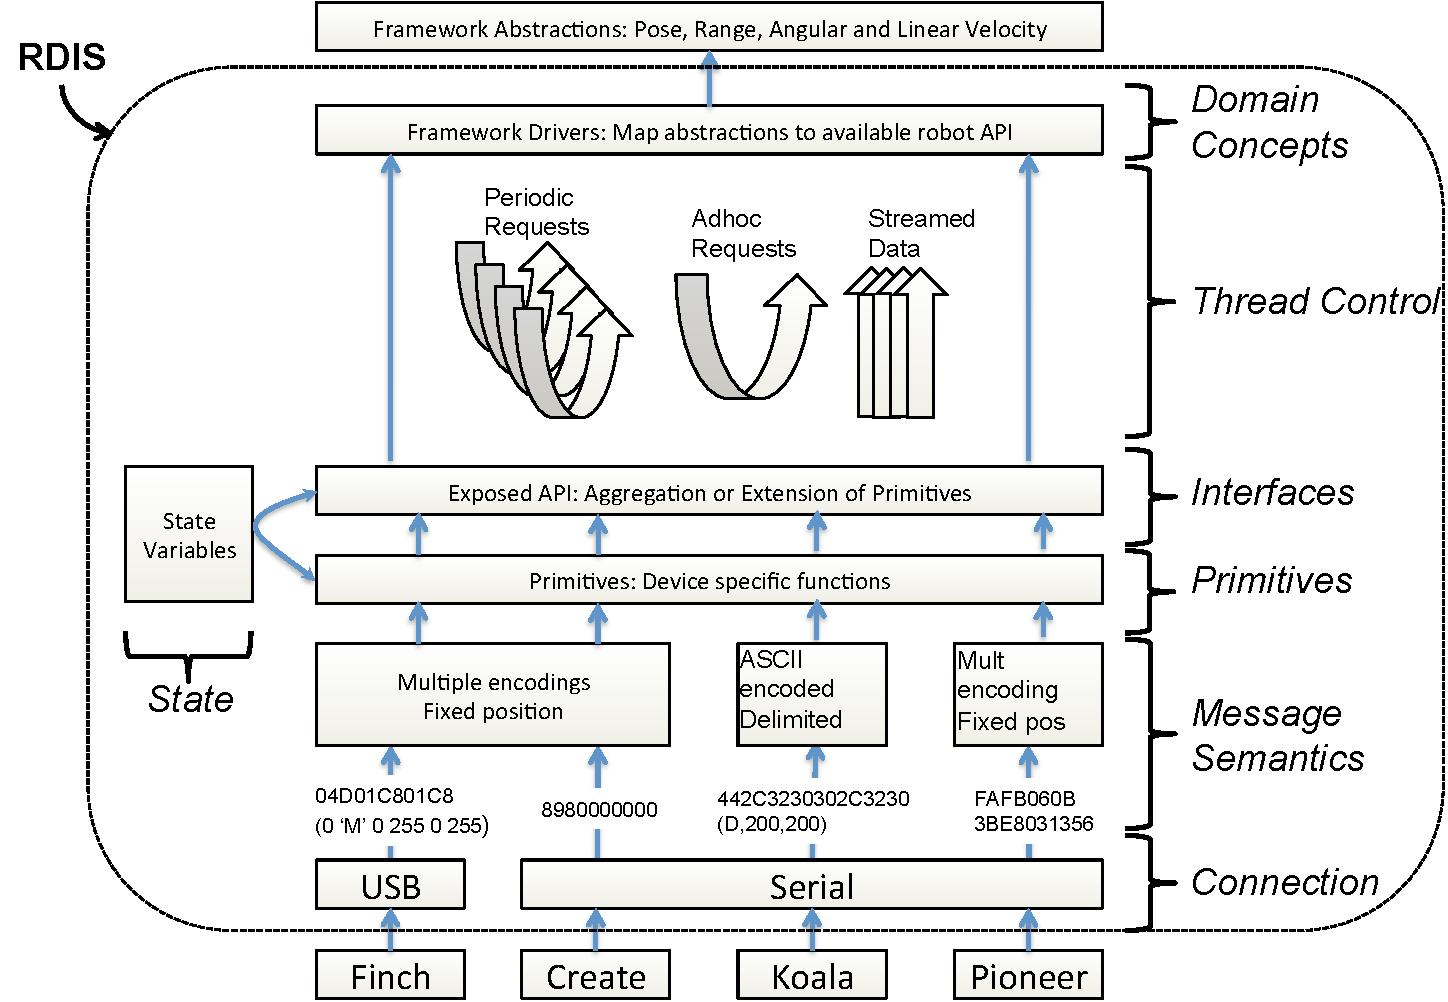
\includegraphics[width=5in]{dm.pdf}
      \caption{Preliminary domain model for mapping devices to frameworks.}
      \label{dm}
\end{figure*}

This preliminary result supports the idea that general robot devices can be described declaratively in a manner that supports discovery and that links to the backend processes.  The RDIS must be expanded to be useful in a larger context.  The work proposed as part of this effort will accomplish the following major innovations to RDIS as a contribution to the engineering of cyber-physical systems: 
\begin{enumerate}
\item Extend the processing models to include a larger set of execution semantics, 
\item Extend the actuation model to include a larger set of popular kinematic chains from both manufacturing and exploration robotics, and
\item Using RDIS as a hardware discovery mechanism, show composition of devices into a controller that is error-aware.   
\end{enumerate}

\subsection{Expansion of execution semantics}

The ability to generalize device to framework mapping requires documenting the concepts in existing mappings.  The domain model captures the invariant features of the device to framework mapping drives the contents of RDIS.  In Figure \ref{dm}, the domain is broken into seven related concepts: 1) connections, 2) state, 3) message semantics, 4) primitives, 5) interfaces, 6) thread control, and 7) robotics domain concepts.  {\sc Connection} refers to the transport used to communicate from the device driver to the framework.  Information needed to establish and maintain the connection is defined within this concept. The {\sc State} definition serves two purposes: 1) define constants relevant to other sections and 2) allow for state to be saved and retrieved as part of adhoc and periodic requests.   The {\sc Message Semantics} refers to the structure of the data which is actually sent to the robot over the connection. This specification is decided by the manufacturer and is generally uniform between primitives.   {\sc Primitives} focuses on describing the firmware interface in order to document the invariant features of the device.   The {\sc Interface} declaration, acting as a logical view of the {\sc Primitives},  specifies functions that are available to a developer to control a robot.   {\sc Domain Concepts} map interfaces to domain specific concepts in a framework agnostic manner.  These concepts are discussed in detail in \cite{Anderson2012}.

\begin{figure*}[thpb]
      \centering
      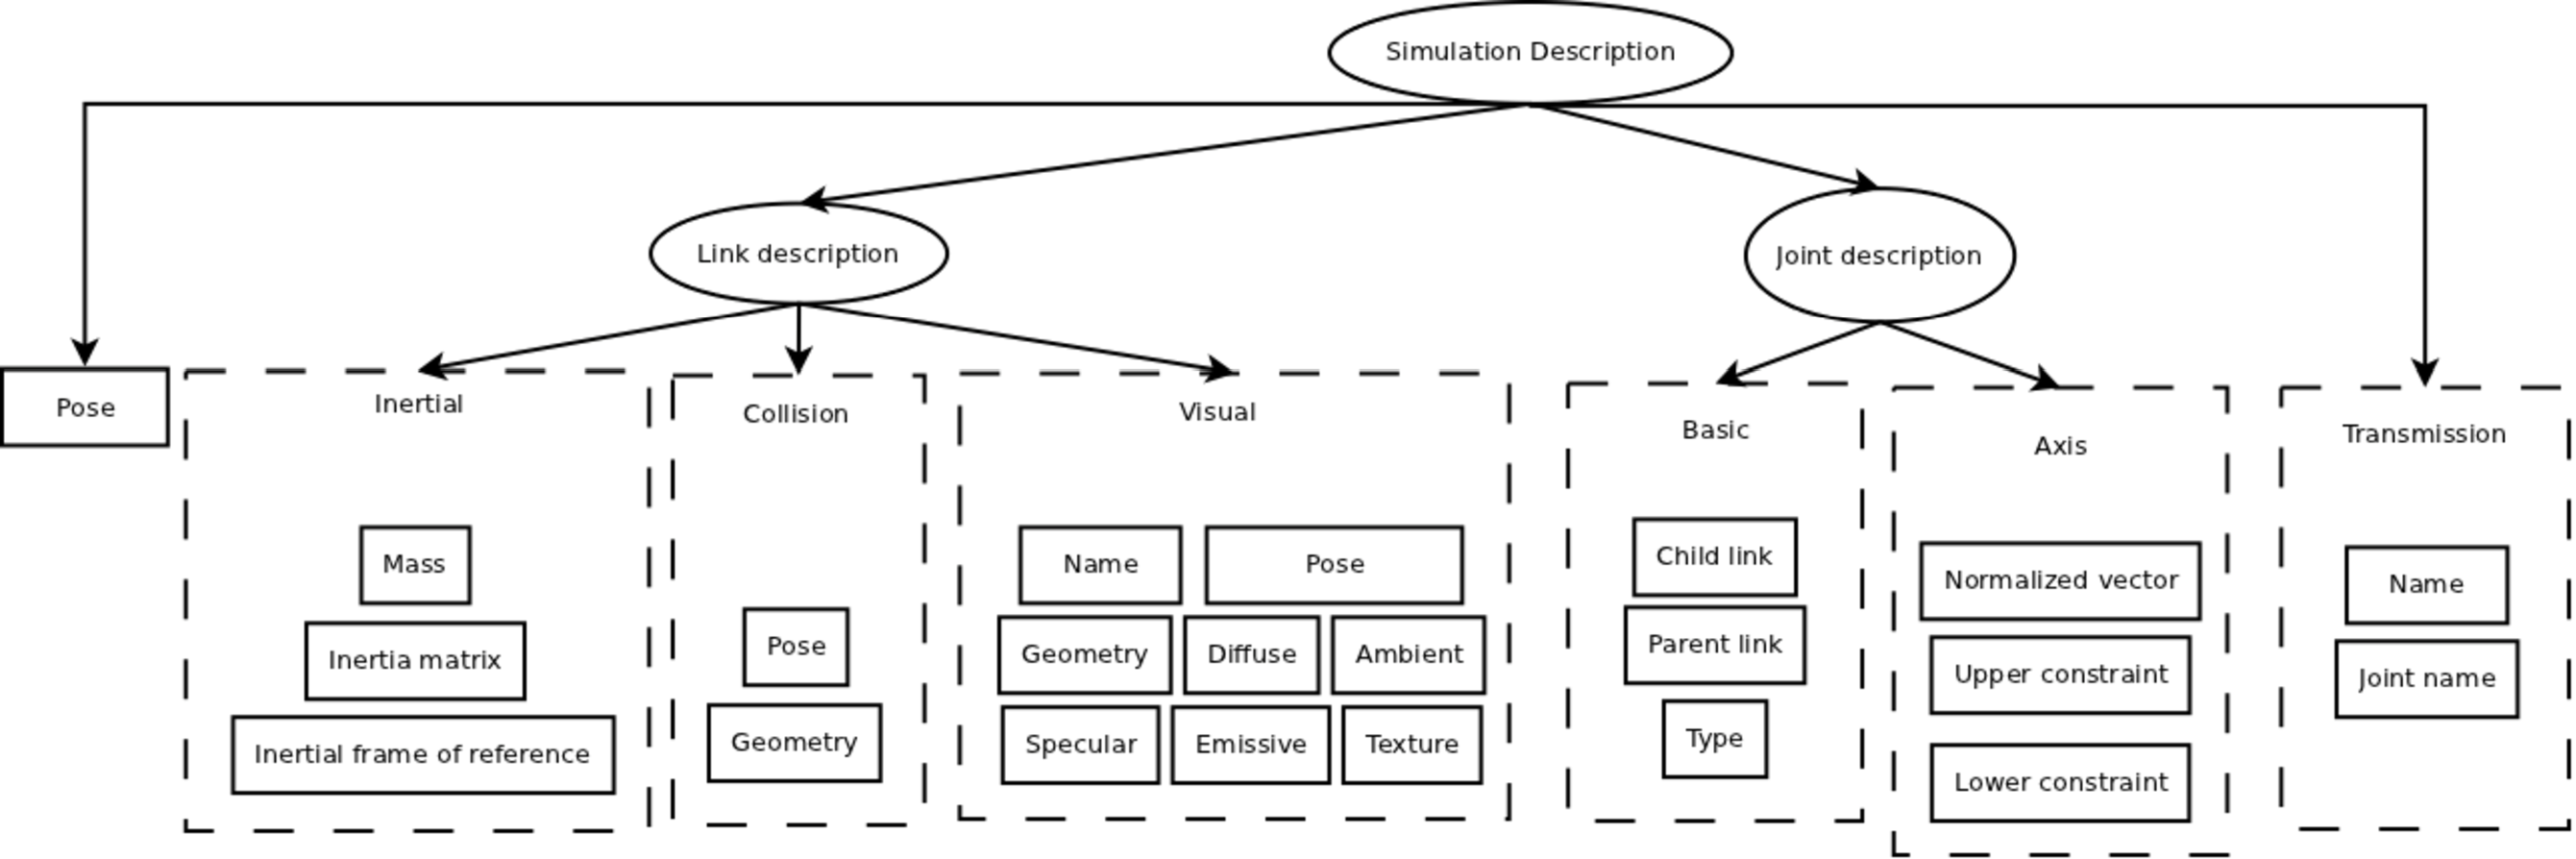
\includegraphics[width=6in]{kvc.pdf}
      \caption{General model for describing kinematics, appearance, collision and dynamics parameters sufficient for simulation on any simulation platform.  Currently targeted platforms include Gazebo, Webots, and ROS.}
      \label{kvc}
\end{figure*}

%These changes require updates to the specification and the underlying set of generation and utilizing tools. 

In this research, we expand the basic implementation of each concept to accommodate a larger set of embedded firmware controllers.  These tasks include: 
\begin{enumerate}
\item Addition of a complete kinematic, visual and collision description consistent with existing simulators and frameworks (see Figure \ref{kvc}).  Although initial focus will be upon the initial kinematic design (differential drive), the proposed model is designed to accommodate other kinematic designs.
\item Standard mechanism for error handling and notification at both the communication and primitive levels.  Error handling examples include re-establishment of connection or actions to take based on output parameters.  This is particularly relevant to platforms that require a heartbeat request periodically.
\item Expansion of the initial single-threaded implementation to include dual and multi-threading models.  A dual model accommodates different input and output threads while a multithreaded model support different frequencies for periodically submitted requests. 
\item Refinement of the state concept and how it matches to primitives and interfaces would provide a scripting language for transformation of data.  The state variable concept is instrumental in implementing periodic requests asynchronously from the client request/reply system.
\item Management of sensor and actuator error models consistent with existing frameworks will allow for manufacturer provided error models to be propagated to the framework or controller.  An example would be a transformation of encoder error to pose error.  Although all sources of error (systematic and non-systematic cannot be accounted for in this approach, it is currently better than existing approaches that abstract out specific device errors.
\end{enumerate}


\subsection{Expansion of domain concepts to additional kinematic chains}
Domain concepts map interfaces to domain specific concepts in a framework agnostic manner.  Each framework has a notion of a general set of abstract data types generated from device drivers such as pose estimates, pose relative to an identified landmark, control via linear and angular velocity along a dimension or axis, and point and fields of open distance.  The {\sc Domain concepts} definition identifies interfaces that map to the abstract concepts allowing for templates to map the abstract concepts to the existing interfaces available on a device.

From the previous sections it is apparent that the robot kinematic modeling languages are missing necessary components for a generalized description for use in simulation. Some description formats do well in defining the geometries of the robot, but make categorical assumptions about the kinematics of the robot, offloading the actual kinematic description to the framework itself. For example. As an example, Stage has a drive ``diff'' statement to label a position element as having differential-drive steering, and Webots has a DifferentialWheels node which acts as the base node of a robot description having differential steering. URDF solves this by defining a relationship between transmissions and joints, but its approach is specific to the PR2 robot.

Current models of kinematics are adept at modeling the construction of the robot in a way that is almost a standard. However, what is missing between all of them is how to model controllable joints. If a solid mapping can be defined between programming interfaces and resultant efforts at joints, this would benefit the robotics community greatly as there is not currently a description format which does so without the aid of a companion plugin or hardware description. RDIS would benefit much from this component as well as it would define the bridge between the control model introduced in earlier work [1], [2] and the kinematic model which it currently lacks. Thus, the work that needs to be done is to define RDIS's kinematic model according to the trends seen from other frameworks and then provide a mapping from interfaces in the control model to transmission efforts at joints in the kinematic model. It is clear that a viable robot kinematic model will somehow take heed of some of the existing description formats to ensure there is sufficient compatibility with the model. The problem lies in deciding which parameters are essential to a proper kinematic modeling and which are parameters which lose meaning when carried to other frameworks. An additional goal is to find a concise set of these parameters such that no one parameter may be defined in terms of other parameters. It is necessary for this robot model to follow the link-joint model because it is a well understood and well-established concept within the robotics community from which much of its theory is based [6]. With the adoption of this model it is clear that the major components in the model are LINK and JOINT. These two main components will be defined and the necessary problems associated with each will be reviewed. As well, the possibility of modeling a TRANSMISSION component will be discussed.

Because of the strength of the model, LINK and JOINT have already been examined extensively from many different viewpoints, resulting in a mature description of each of these components in just URDF or SDF. It is the author's opinion that these components are described well by these formats and there is not much to discover save for minute details. For these components a description is offered of how SDF and URDF accomplish their description.

\subsubsection{Link}
The LINK is an atomic rigid body in the robot's structure which constitutes the majority of the robot's composure by mass. A link is a primary parameter to the physics simulation as it contains the parameters necessary to simulate the physics of a robot. Additionally, a simulator typically has a visual representation of the robot to present to the user and a LINK will represent the majority of the visualization, so there will be parameters which are to be used by the simulation renderer. Finally, as the LINK is the only material component in the robot model, it will serve as the basis for the collision model, so the parameters to the collision engine must also be defined.

\begin{enumerate}
\item The {\sc physics} component of the description of LINK defines the parameters needed for physics simulation. This will include the robot mass, rotational inertia matrix, and the inertial frame of reference. This portion of the model is consistent in frameworks which simulate the dynamics of robots. SDF introduces a linear and angular velocity damping in this component, however it was alone in this specification. As the implementation proceeds, it will be apparent if this component is missing any parameters.

\item The {\sc collision} component describes the parameters needed by the collision engine. Generally in most simulation description formats, the main components were the pose of the collision model and the simple geometry which defines it. This is to be differentiated from the visual geometry, as it is not necessarily true that a collision geometry may be used as a visual geometry or vice-versa. For instance, Webots uses an IndexedFaceSet type to represent complex or high-fidelity geometries for the visual component of a robot, however this complex type of geometry would be a strain for the collision engine so it is not available for use as a collision geometry. A challenge in defining this component is deciding which collision geometries will effectively represent most robots. 

\item The {\sc visual} component describes the parameters provided to the scene rendering engine. Visual representations are most easily characterized by some sort of geometry, which tended to be the observed pattern within most simulation frameworks. It should be noted that not all frameworks separate the collision model and the visual model. In this case, it usually marks that the simulator is simplistic and does not provide a high definition visual representation of the simulation. In these cases, one geometry is defined to serve as both the collision and visual geometry. In the context of our model, the collision geometry should be selected as it is assumed to be the most simplistic. Solving the collision geometry problem should also determine at least a subset of visual geometries. An additional challenge to defining the visual component will be handling mesh types. Between Webots and Gazebo, there are mesh types ranging from the standard triangle mesh to polygon meshes to height maps. As well, if meshes are supported they are best referenced as they will cloud the description file. 
\end{enumerate}

\subsubsection{Joint} 
The JOINT component of the model characterizes a set of constraints imposed on two joints. In this relationship, there is strictly one related parent LINK and one child LINK. There are six degrees of freedom between two unconstrained links, and a joint restrains one or many of them. The standard degrees of freedom are X, Y, Z, roll, pitch, and yaw. From the examined frameworks, three main types of joints reappear between frameworks, all of which JOINT generalizes a prismatic joint constrains all degrees of freedom except for Z. This allows child link to translate freely in one dimension with respect to the parent link's frame. By convention, this is normally the Z-axis in joint space. This type of joint might be used to model a gripper for a robot arm.

A hinge joint constrains all degrees of freedom except for pitch. This allows a link to rotate in one dimension about a single point of rotation with respect to its parent link's frame. This type of joint might be used to model a fixed wheel on a differential drive robot if no bounds were posed on the joint rotation.  A ball-and-socket joint constrains X, Y, and Z. This allows for rotation of a link about any of its axes with respect to its parent link. This type of joint might be used to model a spherical caster wheel for a differential drive robot.

\subsubsection{Transmission}
A TRANSMISSION component is not yet well-defined in the current state-of-the-art in robot modeling, therefore it may contain some parameters which are to be discovered. From the previously discussed frameworks, URDF was the only description format which included this component, which the documentation notes was not intended to be used for anything but the PR2 robot. Generally speaking, it is known that a transmission is supposed to define how a motor applies effort to a joint or several joints. Therefore, it can be concluded that a transmission must have an association with at least one joint.

Additionally, transmissions mark a point of control for the robot application. If an application wishes to command a robot to move in some manner, then the application must utilize the appropriate interfaces, which in turn triggers one or more robot control primitives which alter the state of the joints. Therefore, a primitive must somehow relate to some transmission and subsequently the parameters provided to the primitive. For example, it could be possible to translate a motor speed to the effort applied at that joint declaratively, and this might require a modification to the previously mentioned control model at the PRIMITIVE component. 

With the major components of the model identified via a survey of existing frameworks, what remains is to discover which components are required to produce a full implementation of the RDIS model. To that end, further research is required. At this point, the relationship between the kinematic model and the control model have been established. The specifics of what is contained in the kinematic and control packages is within the scope of this project. The control model is expected to change slightly to provide support for manipulation of the kinematic model during simulation, while the kinematic model will be wholly new to RDIS while the bindings between the control model and the kinematic model will be clearly defined as a contribution to the robotics modeling community.

\subsection{RDIS-enabled tools}
{\bf talk about how we can use rids to assist with development of controller by using existing tools for domain modeling}
